\documentclass{beamer}
\usepackage{tikz}
\usetikzlibrary{shapes,calc}
\begin{document}

\begin{frame}
\center
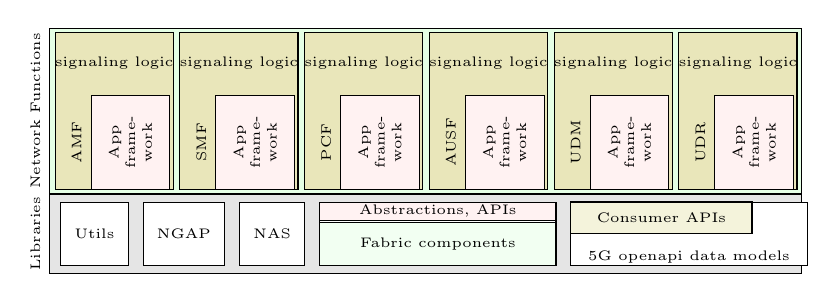
\begin{tikzpicture}[nf/.style={rectangle, draw, fill=olive!20,minimum width=1.5cm, minimum height=2cm},
app/.style={rectangle, draw, fill=red!5,minimum width=1cm, minimum height=1.2cm},
libc/.style={rectangle, draw, fill=white,minimum height=0.8cm, inner sep=5pt,font=\tiny},
lab/.style={inner sep=1pt,align=center, font=\tiny}]

\node[rectangle,draw,fill=green!10, minimum width=9.55cm, minimum height=2.1cm] at (0,0) (app) {};
\node[rectangle,draw,fill=black!10, minimum width=9.55cm, minimum height=1cm,below] at (app.south) (lib) {};

\node[lab, rotate=90] at ([xshift=-5pt]app.west) {Network Functions}; 
\node[lab, rotate=90] at ([xshift=-5pt]lib.west) {Libraries}; 

\node[nf,right] at ([xshift=2pt]app.west) (amf) {};
\node[nf,right] at ([xshift=2pt]amf.east) (smf) {};
\node[nf,right] at ([xshift=2pt]smf.east) (pcf) {};
\node[nf,right] at ([xshift=2pt]pcf.east) (ausf) {};
\node[nf,right] at ([xshift=2pt]ausf.east) (udm) {};
\node[nf,right] at ([xshift=2pt]udm.east) (udr) {};

\node[app,above] at ([xshift=-0.55cm]amf.south east) (amfapp) {}; 
\node[app,above] at ([xshift=-0.55cm]smf.south east) (smfapp) {}; 
\node[app,above] at ([xshift=-0.55cm]pcf.south east) (pcfapp) {}; 
\node[app,above] at ([xshift=-0.55cm]ausf.south east) (ausfapp) {}; 
\node[app,above] at ([xshift=-0.55cm]udm.south east) (udmapp) {}; 
\node[app,above] at ([xshift=-0.55cm]udr.south east) (udrapp) {}; 

\node[lab,rotate=90,text width=1cm, align=center, inner sep=0] at (amfapp) {App framework};
\node[lab, rotate=90] at ([xshift=-5pt]amfapp.west) {AMF};
\node[lab, below] at ([yshift=-8pt]amf.north) {signaling logic};

\node[lab,rotate=90,text width=1cm, align=center, inner sep=0] at (smfapp) {App framework};
\node[lab, rotate=90] at ([xshift=-5pt]smfapp.west) {SMF};
\node[lab, below] at ([yshift=-8pt]smf.north) {signaling logic};

\node[lab,rotate=90,text width=1cm, align=center, inner sep=0] at (pcfapp) {App framework};
\node[lab, rotate=90] at ([xshift=-5pt]pcfapp.west) {PCF};
\node[lab, below] at ([yshift=-8pt]pcf.north) {signaling logic};

\node[lab,rotate=90,text width=1cm, align=center, inner sep=0] at (ausfapp) {App framework};
\node[lab, rotate=90] at ([xshift=-5pt]ausfapp.west) {AUSF};
\node[lab, below] at ([yshift=-8pt]ausf.north) {signaling logic};

\node[lab,rotate=90,text width=1cm, align=center, inner sep=0] at (udmapp) {App framework};
\node[lab, rotate=90] at ([xshift=-5pt]udmapp.west) {UDM};
\node[lab, below] at ([yshift=-8pt]udm.north) {signaling logic};

\node[lab,rotate=90,text width=1cm, align=center, inner sep=0] at (udrapp) {App framework};
\node[lab, rotate=90] at ([xshift=-5pt]udrapp.west) {UDR};
\node[lab, below] at ([yshift=-8pt]udr.north) {signaling logic};

\node[libc,right] at ([xshift=4pt]lib.west) (utils) {Utils};
\node[libc,right] at ([xshift=5pt]utils.east) (ngap) {NGAP};
\node[libc,right] at ([xshift=5pt]ngap.east) (nas) {NAS};
\node[libc,right, minimum width=3cm] at ([xshift=5pt]nas.east) (fabric) {};
\node[libc,right, minimum width=3cm] at ([xshift=5pt]fabric.east) (openapi) {};
\node[lab,below, draw, fill=red!5, minimum width=3cm] at (fabric.north) {Abstractions, APIs};
\node[lab,above, draw, fill=green!5, minimum width=3cm, minimum height=0.55cm] at (fabric.south) {Fabric components};
\node[lab, draw, fill= olive!10, right, minimum height=0.4cm, minimum width=2.3cm] at ([yshift=-0.2cm]openapi.north west) {Consumer APIs};
\node[above,lab] at (openapi.south) {5G openapi data models};
\end{tikzpicture}


\end{frame}

\end{document}